\phantomsection
\section*{Глава 2. Проектирование веб-приложения}
\addcontentsline{toc}{section}{Глава 2. Проектирование веб-приложения}
\stepcounter{section}

\subsection{Анализ целевой аудитории}

Разрабатываемое веб-приложение предназначено для небольшой библиотеки, в которой
основными процессами являются учет книг, регистрация читателей, оформление выдачи
и возврата книг, поиск изданий и получение простой статистики. Приложение
предполагает работу через браузер, поэтому пользователю не требуется устанавливать
отдельную клиентскую программу на рабочий компьютер.

Основными пользователями системы являются:

\begin{itemize}
    \item \textbf{Библиотекарь} --- сотрудник библиотеки, ответственный за ведение
          книжного фонда, регистрацию читателей, оформление выдачи и возврата
          книг, а также просмотр статистики.

    \item \textbf{Читатель} --- пользователь библиотеки, которому необходимо
          просматривать каталог книг, искать нужные издания и отслеживать
          информацию о собственных выдачах.

    \item \textbf{Администратор} --- технический пользователь, отвечающий за
          управление учетными записями, назначение ролей и контроль работы
          приложения.
\end{itemize}

В небольшой библиотеке роли администратора и библиотекаря могут выполняться одним
сотрудником. При этом в проектируемой системе они разделяются логически:
администратор отвечает за учетные записи, роли и права доступа, а библиотекарь
работает с предметными данными --- книгами, читателями и выдачами. Один
пользователь системы может иметь несколько ролей одновременно, поэтому сотруднику,
совмещающему обязанности администратора и библиотекаря, не требуется создавать
две отдельные учетные записи. Такое разделение позволяет сохранить простую
структуру приложения и одновременно явно определить границы доступа пользователей.

Для библиотекаря основными потребностями являются быстрый доступ к операциям
добавления и редактирования книг, оформление выдач, контроль возвратов и получение
сводной информации о состоянии фонда. Для читателя важны простота поиска,
доступность каталога и возможность видеть сведения о выданных ему книгах.
Администратор обеспечивает техническую настройку системы и разграничение прав
доступа.

Таким образом, интерфейс приложения должен быть разделен по ролям. Библиотекарь
получает доступ к разделам управления книгами, читателями и журналом выдач.
Читатель получает доступ к каталогу и личной информации о выдачах. Администратор
получает доступ к управлению пользователями и ролями.

\subsection{Описание функциональности приложения}

Функциональность веб-приложения определяется основными процессами библиотеки.
Система должна обеспечивать учет книг, учет читателей, оформление выдачи и
возврата книг, поиск и фильтрацию записей, формирование статистики, а также
загрузку обложек книг и выгрузку данных.

Основной пользовательский сценарий для библиотекаря можно сформулировать в виде
\textit{User Story}: «Я, как библиотекарь, хочу вести электронный каталог книг и
журнал выдач, чтобы быстро находить информацию о книгах, читателях и текущем
состоянии фонда».

Для читателя основной пользовательский сценарий формулируется следующим образом:
«Я, как читатель, хочу просматривать каталог и искать книги по названию, автору
или категории, чтобы заранее узнать, есть ли нужное издание в библиотеке».

Основные функции приложения:

\begin{itemize}
    \item регистрация и вход пользователей в систему;
    \item разграничение прав доступа для ролей <<библиотекарь>>, <<читатель>> и
          <<администратор>>;
    \item просмотр каталога книг;
    \item поиск и фильтрация книг по названию, автору, категории и доступности;
    \item добавление, просмотр, редактирование и удаление записей о книгах;
    \item самостоятельная регистрация читателей, просмотр и редактирование их данных библиотекарем;
    \item оформление выдачи книги читателю;
    \item оформление возврата книги;
    \item просмотр журнала выдач;
    \item формирование статистики по книгам, читателям и выдачам;
    \item загрузка обложек книг при добавлении или редактировании записей;
    \item выгрузка данных в CSV для формирования отчетов.
\end{itemize}

При проектировании функциональности необходимо учитывать, что часть действий
доступна только после входа пользователя в систему. В частности, просмотр личных
выдач доступен только авторизованному читателю, так как система должна определить,
к какой учетной записи относится пользователь. Аналогично, операции управления
книгами, читателями, выдачами, обложками книг и статистикой доступны только пользователю
с ролью библиотекаря.

На рисунке~\ref{fig:use_case} представлена диаграмма вариантов использования
разрабатываемого веб-приложения.

\begin{figure}[H]
    \centering
    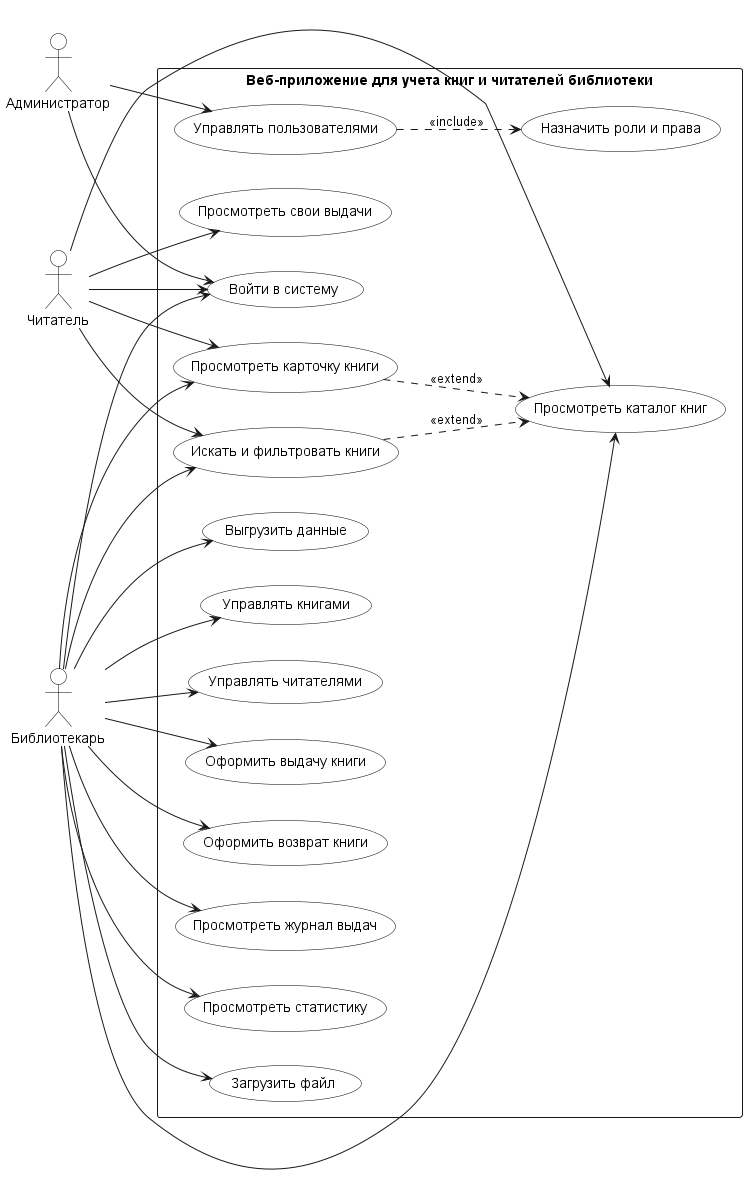
\includegraphics[width=0.95\textwidth]{images/use_case.png}
    \caption{Диаграмма вариантов использования веб-приложения}
    \label{fig:use_case}
\end{figure}

Вариант использования <<Загрузить файл>> в рамках разрабатываемого приложения
предполагает загрузку обложки книги при добавлении или редактировании записи о
книге. Файл обложки сохраняется в каталоге пользовательских медиафайлов, а в
записи о книге хранится путь к изображению.

Вариант использования <<Выгрузить данные>> означает экспорт сведений из системы
во внешний файл. В рамках приложения такая функция используется для выгрузки
каталога книг и журнала выдач в CSV.

Следует также различать управление читателями и управление пользователями.
Вариант использования <<Управлять читателями>> относится к работе библиотекаря с
карточками читателей: просмотру списка читателей, редактированию ФИО, контактных
данных и просмотру информации о выданных книгах. Вариант использования <<Управлять
пользователями>> относится к действиям администратора с учетными записями,
ролями и правами доступа.


\subsection{Проектирование модели данных}

Для хранения информации используется реляционная модель данных. Основными
сущностями приложения являются книга, читатель и запись о выдаче. Дополнительно
выделяются сущности автора и категории, а также промежуточные сущности для
реализации связей многие ко многим между книгами, авторами и категориями.
Учетные записи пользователей и роли реализуются с использованием встроенных
механизмов Django.

Основные сущности модели данных:

\begin{itemize}
    \item \texttt{User} --- учетная запись пользователя системы;
    \item \texttt{Reader} --- читатель библиотеки;
    \item \texttt{Author} --- автор книги или авторский коллектив;
    \item \texttt{Category} --- категория книги;
    \item \texttt{Book} --- конкретное издание книги библиотечного фонда;
    \item \texttt{BookAuthor} --- связь книги и автора;
    \item \texttt{BookCategory} --- связь книги и категории;
    \item \texttt{Loan} --- запись о выдаче книги.
\end{itemize}

Отдельная сущность для универсального хранения загруженных файлов в модели данных
не используется. Загрузка файлов в приложении реализуется как загрузка обложки
книги: путь к файлу хранится в поле \texttt{cover} сущности \texttt{Book}. Такой
подход проще и точнее соответствует предметной области, так как обложка является
атрибутом конкретного издания.

Связи между сущностями определяются логикой предметной области. Один автор может
быть связан с несколькими книгами, а одна книга может иметь нескольких авторов.
Для реализации такой связи используется промежуточная сущность
\texttt{BookAuthor}. Одна книга может относиться к нескольким категориям, а одна
категория может использоваться для классификации нескольких книг; эта связь
реализуется через сущность \texttt{BookCategory}. Один читатель может иметь
несколько записей о выдаче. Одна книга может многократно фигурировать в журнале
выдач, так как она может выдаваться разным читателям в разные периоды времени.

На рисунке~\ref{fig:er_diagram} представлена ER-диаграмма модели данных.

\begin{figure}[H]
    \centering
    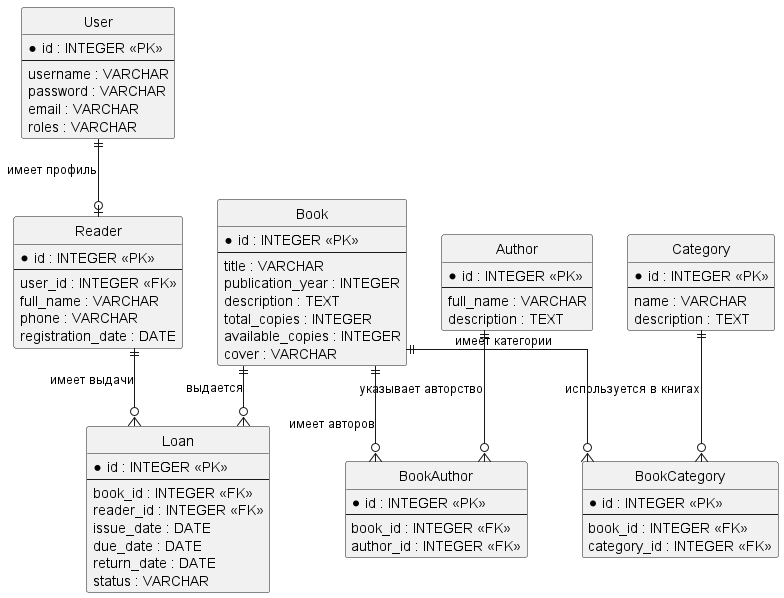
\includegraphics[width=0.95\textwidth]{images/er_diagram.png}
    \caption{ER-диаграмма модели данных}
    \label{fig:er_diagram}
\end{figure}

На ER-диаграмме первичные ключи сущностей обозначены как \texttt{PK}, а внешние
ключи --- как \texttt{FK}. Связи между сущностями показывают логические отношения
между объектами предметной области. Конкретные соответствия первичных и внешних
ключей дополнительно раскрываются в логической и физической схемах базы данных,
представленных в табл.~\ref{tab:logical_schema} и табл.~\ref{tab:physical_schema}.

Сущность \texttt{User} используется для хранения учетных записей пользователей:
логина, пароля, электронной почты и ролей. В логической модели поле
\texttt{roles} отражает набор ролей пользователя. В реализации на Django
разграничение доступа выполняется с использованием встроенных групп и прав.
Такой подход позволяет назначать одному пользователю несколько ролей
одновременно, например роли библиотекаря и администратора.

Сущность \texttt{Reader} описывает карточку читателя библиотеки и связана с
учетной записью пользователя через внешний ключ \texttt{user\_id}. Такое
разделение позволяет отдельно хранить данные, необходимые для входа в систему, и
предметные данные читателя: ФИО, телефон и дату регистрации.

Связь между сущностями \texttt{User} и \texttt{Reader} имеет тип один к нулю или
одному. Не каждая учетная запись пользователя является учетной записью читателя:
пользователи с ролями администратора и библиотекаря могут не иметь карточки
читателя. При этом карточка читателя, если она создана, связана только с одной
учетной записью пользователя.

Отдельные сущности для библиотекаря и администратора в модели данных не
выделяются, так как данные пользователи отличаются прежде всего набором прав
доступа. Их учетные записи хранятся в сущности \texttt{User}, а доступ к функциям
системы определяется ролью пользователя.

Сущность \texttt{Author} используется для хранения сведений об авторах книг.
Автором может быть как отдельный человек, так и авторский коллектив или
организация. Поскольку одна книга может иметь нескольких авторов, а один автор
может быть связан с несколькими книгами, связь между сущностями \texttt{Author}
и \texttt{Book} реализуется как связь многие ко многим через промежуточную
сущность \texttt{BookAuthor}.

Сущность \texttt{Book} используется для хранения сведений о конкретном издании
книги: названии, годе издания, описании, количестве экземпляров и файле обложки.
В каталоге несколько изданий одного произведения могут отображаться как
обобщенная запись с возможностью раскрытия списка изданий. При этом на уровне
базы данных каждое издание хранится как отдельная запись сущности \texttt{Book}.

Связь между книгами и категориями также является связью многие ко многим: одна
книга может относиться к нескольким категориям, а одна категория может
использоваться для классификации нескольких книг. Для реализации такой связи
выделена промежуточная сущность \texttt{BookCategory}, которая связывает записи
\texttt{Book} и \texttt{Category} через внешние ключи \texttt{book\_id} и
\texttt{category\_id}.

Сущность \texttt{Loan} используется для хранения записей о выдаче книг. Она
связана с сущностью \texttt{Reader} через внешний ключ \texttt{reader\_id}, а с
сущностью \texttt{Book} --- через внешний ключ \texttt{book\_id}. Благодаря этому
один читатель может иметь несколько записей о выдаче, а одна книга может
многократно встречаться в журнале выдач в разные периоды времени.

Логическая схема базы данных представлена в табл.~\ref{tab:logical_schema}.

{
\coursetablesetup
\setlength{\LTleft}{0pt}
\setlength{\LTright}{0pt}

\begin{longtable}{|
p{\dimexpr0.18\textwidth-2\tabcolsep-\arrayrulewidth\relax}|
p{\dimexpr0.43\textwidth-2\tabcolsep-\arrayrulewidth\relax}|
p{\dimexpr0.39\textwidth-2\tabcolsep-\arrayrulewidth\relax}|}
    \caption{Логическая схема базы данных}
    \label{tab:logical_schema} \\

    \hline
    \textbf{Сущность} & \textbf{Атрибуты} & \textbf{Связи} \\ \hline
    \endfirsthead

    \tabcont{\ref{tab:logical_schema}}
    \textbf{Сущность} & \textbf{Атрибуты} & \textbf{Связи} \\ \hline
    \endhead

    \hline
    \endfoot

    User &
    id, username, password, email, roles &
    Один к нулю или одному с Reader \\ \hline

    Reader &
    id, user\_id, full\_name, phone, registration\_date &
    Один к одному с User; один ко многим с Loan \\ \hline

    Author &
    id, full\_name, description &
    Один ко многим с BookAuthor \\ \hline

    Category &
    id, name, description &
    Один ко многим с BookCategory \\ \hline

    Book &
    id, title, publication\_year, description, total\_copies, available\_copies, cover &
    Один ко многим с BookAuthor; один ко многим с BookCategory; один ко многим с Loan \\ \hline

    BookAuthor &
    id, book\_id, author\_id &
    Многие к одному с Book; многие к одному с Author \\ \hline

    BookCategory &
    id, book\_id, category\_id &
    Многие к одному с Book; многие к одному с Category \\ \hline

    Loan &
    id, book\_id, reader\_id, issue\_date, due\_date, return\_date, status &
    Многие к одному с Book; многие к одному с Reader \\ \hline
\end{longtable}
}

Физическая схема базы данных будет реализована с использованием моделей Django.
Для основных полей будут применяться типы данных, соответствующие возможностям
ORM Django и SQLite. Предварительная структура ключевых таблиц представлена в
табл.~\ref{tab:physical_schema}.

{
\coursetablesetup
\setlength{\LTleft}{0pt}
\setlength{\LTright}{0pt}

\begin{longtable}{|
p{\dimexpr0.31\textwidth-2\tabcolsep-\arrayrulewidth\relax}|
p{\dimexpr0.23\textwidth-2\tabcolsep-\arrayrulewidth\relax}|
p{\dimexpr0.46\textwidth-2\tabcolsep-\arrayrulewidth\relax}|}
    \caption{Физическая схема основных таблиц}
    \label{tab:physical_schema} \\

    \hline
    \textbf{Поле} & \textbf{Тип данных} & \textbf{Описание} \\ \hline
    \endfirsthead

    \tabcont{\ref{tab:physical_schema}}
    \textbf{Поле} & \textbf{Тип данных} & \textbf{Описание} \\ \hline
    \endhead

    \hline
    \endfoot

    \multicolumn{3}{|l|}{\textbf{Таблица readers}} \\ \hline
    id & INTEGER & Первичный ключ \\ \hline
    user\_id & INTEGER & Уникальный внешний ключ на пользователя \\ \hline
    full\_name & VARCHAR(255) & ФИО читателя \\ \hline
    phone & VARCHAR(20) & Телефон читателя \\ \hline
    registration\_date & DATE & Дата регистрации читателя \\ \hline

    \multicolumn{3}{|l|}{\textbf{Таблица authors}} \\ \hline
    id & INTEGER & Первичный ключ \\ \hline
    full\_name & VARCHAR(255) & ФИО автора или название авторского коллектива \\ \hline
    description & TEXT & Краткая информация об авторе \\ \hline

    \multicolumn{3}{|l|}{\textbf{Таблица categories}} \\ \hline
    id & INTEGER & Первичный ключ \\ \hline
    name & VARCHAR(100) & Название категории \\ \hline
    description & TEXT & Описание категории \\ \hline

    \multicolumn{3}{|l|}{\textbf{Таблица books}} \\ \hline
    id & INTEGER & Первичный ключ \\ \hline
    title & VARCHAR(255) & Название книги \\ \hline
    publication\_year & INTEGER & Год издания \\ \hline
    description & TEXT & Описание книги \\ \hline
    total\_copies & INTEGER & Общее количество экземпляров \\ \hline
    available\_copies & INTEGER & Количество доступных экземпляров \\ \hline
    cover & VARCHAR(255) & Путь к файлу обложки \\ \hline

    \multicolumn{3}{|l|}{\textbf{Таблица book\_authors}} \\ \hline
    id & INTEGER & Первичный ключ \\ \hline
    book\_id & INTEGER & Внешний ключ на книгу \\ \hline
    author\_id & INTEGER & Внешний ключ на автора \\ \hline

    \multicolumn{3}{|l|}{\textbf{Таблица book\_categories}} \\ \hline
    id & INTEGER & Первичный ключ \\ \hline
    book\_id & INTEGER & Внешний ключ на книгу \\ \hline
    category\_id & INTEGER & Внешний ключ на категорию \\ \hline

    \multicolumn{3}{|l|}{\textbf{Таблица loans}} \\ \hline
    id & INTEGER & Первичный ключ \\ \hline
    book\_id & INTEGER & Внешний ключ на книгу \\ \hline
    reader\_id & INTEGER & Внешний ключ на читателя \\ \hline
    issue\_date & DATE & Дата выдачи \\ \hline
    due\_date & DATE & Плановая дата возврата \\ \hline
    return\_date & DATE & Фактическая дата возврата \\ \hline
    status & VARCHAR(20) & Статус выдачи \\ \hline
\end{longtable}
}

Для обеспечения целостности данных необходимо предусмотреть ограничения. Количество
доступных экземпляров книги не должно быть отрицательным и не должно превышать
общее количество экземпляров. Запись о выдаче должна быть связана с существующей
книгой и существующим читателем. При оформлении выдачи количество доступных
экземпляров книги должно уменьшаться, а при возврате увеличиваться. Срок возврата
не должен быть раньше даты выдачи.

\subsection{Разработка макетов страниц}

На этапе проектирования определены основные страницы веб-приложения. Макеты
страниц используются для предварительного описания структуры интерфейса до начала
реализации. Они позволяют определить расположение меню, заголовков, форм, таблиц,
кнопок и информационных блоков.

Основные страницы приложения:

\begin{itemize}
    \item страница входа;
    \item главная страница;
    \item каталог книг;
    \item карточка книги;
    \item страница управления книгами;
    \item страница управления читателями;
    \item журнал выдач;
    \item страница статистики;
    \item административный раздел.
\end{itemize}

На рисунке~\ref{fig:login_wireframe} представлен макет страницы авторизации.

\begin{figure}[H]
    \centering
    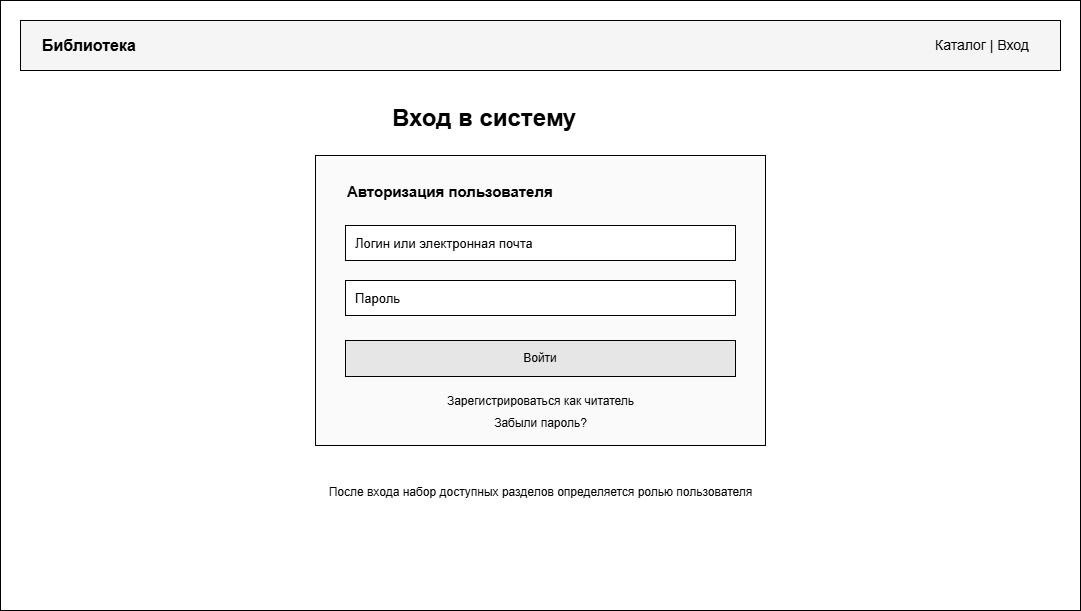
\includegraphics[width=0.85\textwidth]{images/login_wireframe.png}
    \caption{Макет страницы авторизации}
    \label{fig:login_wireframe}
\end{figure}

Страница авторизации предназначена для входа пользователя в систему. Для читателей
также предусматривается переход к форме самостоятельной регистрации. Учетные
записи сотрудников создаются администратором, поэтому регистрация библиотекарей и
администраторов через публичную форму не предусматривается. После успешного входа
набор доступных разделов определяется ролью пользователя.

Ссылка восстановления доступа <<Забыли пароль?>> не отображается на форме
авторизации постоянно. Она появляется только после неудачной попытки входа, когда
пользователь вводит неверный пароль. Такой подход позволяет не перегружать базовый
вид формы авторизации дополнительными элементами, но при этом предоставляет
пользователю возможность восстановить доступ при возникновении проблемы со входом.

На рисунке~\ref{fig:catalog_wireframe} представлен макет страницы каталога книг.

\begin{figure}[H]
    \centering
    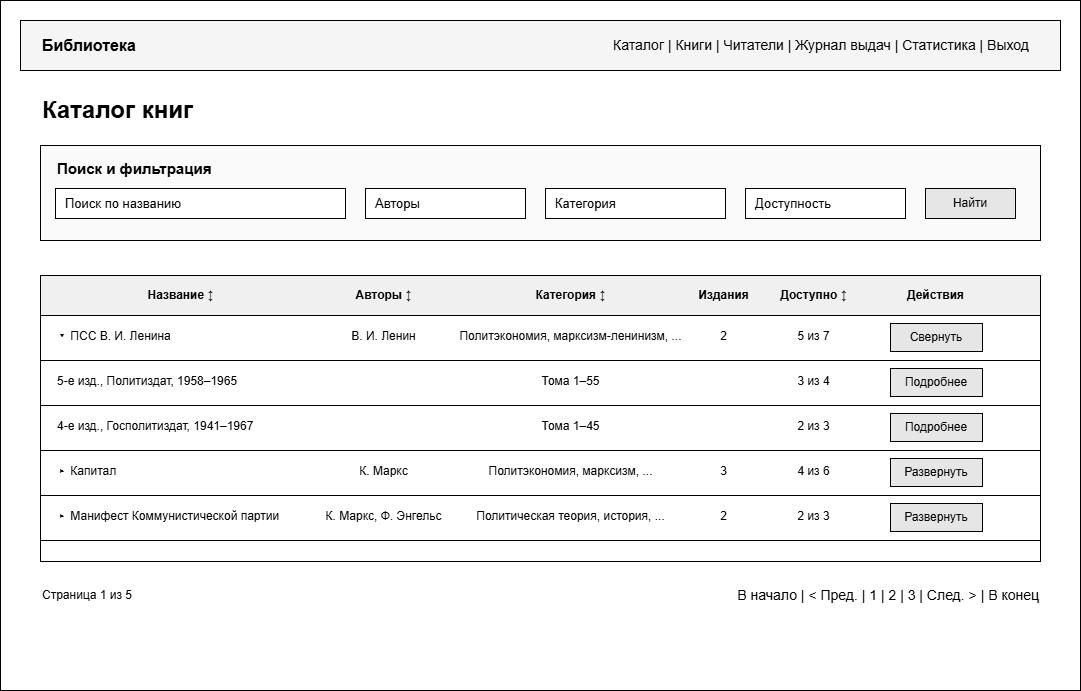
\includegraphics[width=\textwidth]{images/catalog_wireframe.png}
    \caption{Макет страницы каталога книг}
    \label{fig:catalog_wireframe}
\end{figure}

В макете каталога предусмотрены поиск, фильтрация и сортировка записей. Сортировка
выполняется через заголовки столбцов: пользователь может изменить порядок вывода
по названию, автору, категории или количеству доступных экземпляров. Авторы и
категории могут использоваться как элементы быстрого перехода к отфильтрованному
списку книг.

Каталог учитывает наличие разных изданий одного произведения. Обобщенная строка
показывает название произведения и суммарную доступность экземпляров, а при
раскрытии строки отображаются отдельные издания с указанием года издания, состава
томов и доступного количества экземпляров.

В нижней части каталога предусматривается постраничная навигация. Пользователь
может перейти к предыдущей или следующей странице, выбрать конкретный номер
страницы, а также перейти в начало или конец списка.

В списке каталога для книги показываются только основные категории. Если книга
относится к нескольким категориям, в таблице выводятся первые в списке категории и
многоточие, а полный список категорий отображается в карточке книги.

На рисунке~\ref{fig:book_card_wireframe} представлен макет карточки книги.

\begin{figure}[H]
    \centering
    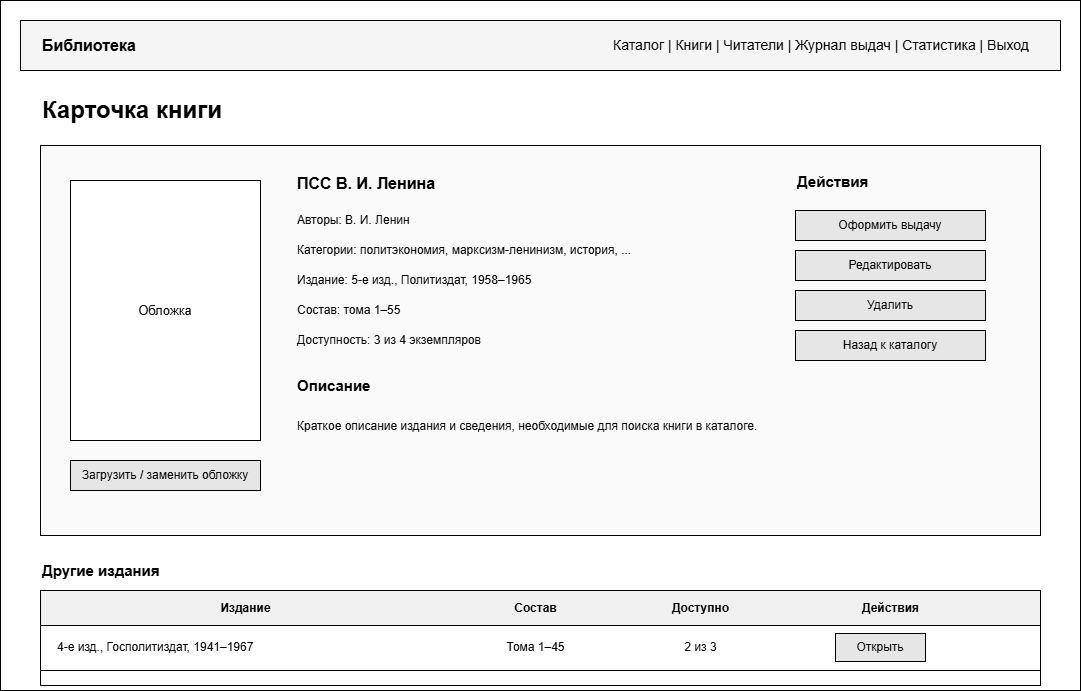
\includegraphics[width=\textwidth]{images/book_card_wireframe.png}
    \caption{Макет карточки книги}
    \label{fig:book_card_wireframe}
\end{figure}

Карточка книги предназначена для просмотра подробной информации о выбранном
издании. На странице отображаются название, авторы, категории, сведения об
издании, доступность экземпляров, обложка и краткое описание. Также предусмотрено
отображение других изданий того же произведения.

Набор элементов на карточке книги зависит от роли пользователя. Кнопки
редактирования записи, удаления книги, загрузки или замены обложки, а также
оформления выдачи доступны только библиотекарю. Для читателя карточка книги
отображается в режиме просмотра: пользователь видит сведения о книге и информацию
о доступности экземпляров, но не имеет доступа к служебным действиям.

На рисунке~\ref{fig:loans_wireframe} представлен макет страницы журнала выдач.

\begin{figure}[H]
    \centering
    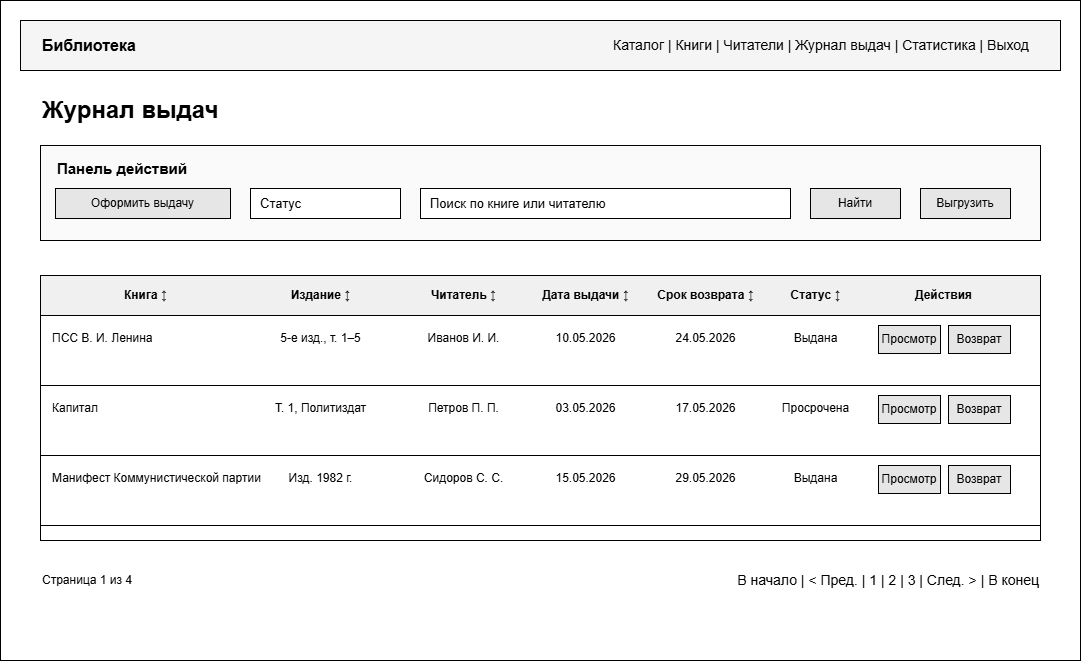
\includegraphics[width=\textwidth]{images/loans_wireframe.png}
    \caption{Макет страницы журнала выдач}
    \label{fig:loans_wireframe}
\end{figure}

Макет страницы журнала выдач отражает основной рабочий сценарий библиотекаря:
поиск записей о выдаче, фильтрацию по статусу, оформление новой выдачи, просмотр
сведений о записи и оформление возврата книги. Для удобства работы в таблице
предусмотрена сортировка по основным столбцам: книге, изданию, читателю, дате
выдачи, сроку возврата и статусу.

В журнале выдач отображается не только название книги, но и конкретное издание,
поскольку выдача оформляется на определенное издание книги. Это позволяет отличать
разные издания одного произведения, например разные издания ПСС В. И. Ленина или
отдельные тома произведения. В нижней части страницы предусматривается
постраничная навигация с переходом в начало и конец списка.

На рисунке~\ref{fig:statistics_wireframe} представлен макет страницы статистики.

\begin{figure}[H]
    \centering
    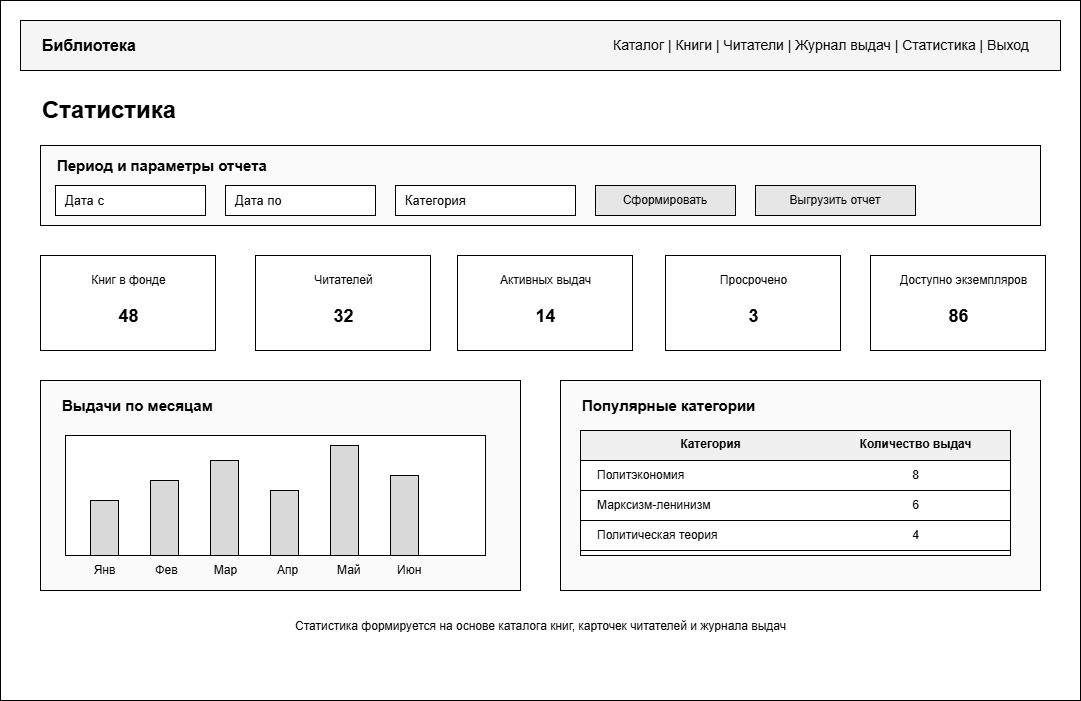
\includegraphics[width=\textwidth]{images/statistics_wireframe.png}
    \caption{Макет страницы статистики}
    \label{fig:statistics_wireframe}
\end{figure}

Страница статистики предназначена для просмотра сводных показателей по состоянию
библиотечного фонда и журналу выдач. На странице отображаются количество книг в
фонде, количество читателей, число активных выдач, количество выдач за все время,
число просроченных возвратов и количество доступных экземпляров.

Также предусмотрена таблица популярных категорий. Для каждой категории могут
отображаться количество книг, количество текущих выдач и количество выдач за все
время. Сортировка таблицы может выполняться по одному из этих показателей. Для
выгрузки данных используется формирование CSV-файлов каталога книг и журнала
выдач.

В результате проектирования определены основные пользователи приложения, описаны
функциональные требования, выделены ключевые сущности модели данных и определены
страницы пользовательского интерфейса. Полученные проектные решения будут
использованы при реализации веб-приложения.
